\documentclass[10pt]{article}
\usepackage{graphicx}
\usepackage{amssymb}
\usepackage{tikz}
\usepackage{epstopdf}
\usepackage{enumitem}
\usepackage{multicol,multirow}
\DeclareGraphicsRule{.tif}{png}{.png}{`convert #1 `dirname #1`/`basename #1 .tif`.png}
\renewcommand{\tablename}{Tabla} 
\renewcommand{\figurename}{Figura} 
\newcommand*\circled[1]{\tikz[baseline=(char.base)]{\node[shape=circle,blue,draw,inner sep=.5pt] (char) {#1};}}

% For a visual definition of these parameters, see
\textwidth = 6.5 in
\textheight = 9 in
\oddsidemargin = 0.0 in
\evensidemargin = 0.0 in
\topmargin = 0.0 in             
\headheight = 0.0 in            
\headsep = 0.0 in
            
\parskip = 0.2in                % vertical space between paragraphs
% Delete the % in the following line if you don't want to have the first line of every paragraph indented
%\parindent = 0.0in

\begin{document}
\begin{center}
    {\Large Pauta Certamen 3, Programaci\'on II} \\
    \emph{\small Prof. Rodrigo Olivares} \\
    \emph{\small Ayud. Diego Agullo} \\
    \emph{\scriptsize Julio 13, 2015}
\end{center}
\vspace*{-35pt}
\begin{center}
    \rule{1\textwidth}{.3pt}
\end{center}
\vspace*{-42pt}
\begin{center}
    \rule{1\textwidth}{2pt}
\end{center}

\vspace*{-15pt}
{\small \textbf{Instrucciones}:}
\vspace*{-15pt}

{\scriptsize
\begin{itemize}
    \item[-] El puntaje m\'aximo del certamen es 100\%, siendo el 60\% el m\'inimo requerido para aprobar.
    \item[-] Responda cada pregunta en la hoja indicada, agregando su nombre. Si no responde alguna pregunta, debe entregar la hoja con su nombre e indicar que \textbf{no responde}.
    \item[-] El certamen es \underline{\textbf{individual}}. Cualquier intento de copia, ser\'a sancionado con nota \textbf{1,0}.
\end{itemize}
\vspace*{10pt}

\vspace*{-30pt}

\begin{enumerate}

    \item \emph{30pts.} De las siguentes afirmaciones, encierre en un c\'irculo la o las alternativas correctas (\emph{3pts c/u}).
    \begin{multicols}{2}

    \begin{enumerate}[label=(\alph*)]
        \item[i.] Un thread: 
        \item[(a)] Es un proceso que se ejecuta en memoria.
        \item[\circled{(b)}] Es un flujo de un proceso en memoria.
        \item[\circled{(c)}] Puede ser creado como clase en Java.
        \item[\circled{(d)}] Puede ser instanciado como objeto.
        \item[(e)] Ninguna de las anteriores.
    \end{enumerate}

    \begin{enumerate}[label=(\alph*)]
        \item[ii.] Para construir una hebra se requiere:
        \item[\circled{(a)}] Extender de una s\'uper clase Thread.
        \item[(b)] Implementar una interfaz Thread.
        \item[(c)] Extender de una s\'uper clase Runneable.
        \item[\circled{(d)}] Implementar una interfaz Runneable.
        \item[(e)] Utilizar el m\'etodo sleep. 
    \end{enumerate}

    \begin{enumerate}[label=(\alph*)]
        \item[iii.] Para una hebra o hilo se debe:
        \item[(a)] Iniciar con el m\'etodo run.
        \item[\circled{(b)}] Iniciar con el m\'etodo start.
        \item[\circled{(c)}] Sobreescribir el m\'etodo run.
        \item[(d)] Sobreescribir el m\'etodo start.
        \item[\circled{(e)}] Instanciar la hebra.
    \end{enumerate}

    \begin{enumerate}[label=(\alph*)]
        \item[iv.] En el ciclo de vida de una hebra, el estado: 
        \item[(a)] New crea e inicializa la hebra.
        \item[\circled{(b)}] Runnable ejecuta la hebra, si hay tiempo CPU asignado.
        \item[(c)] Blocked se ejecuta, sin importar estados internos.
        \item[\circled{(d)}] Dead es invocado generalmente por el m\'etodo stop.
        \item[\circled{(e)}] Yield, verifica el rendimiento del estado Runnable.
    \end{enumerate}

    \begin{enumerate}[label=(\alph*)]
        \item[v.] Un recurso compartido:
        \item[\circled{(a)}] Puede ser una clase.
        \item[\circled{(b)}] Puede ser un objeto de la clase.
        \item[(c)] Puede ser un atributo de la clase.
        \item[\circled{(d)}] Siempre debe estar sincronizado.
        \item[\circled{(e)}] Debe ser declarado como private o protected.
    \end{enumerate}

    \begin{enumerate}[label=(\alph*)]
        \item[vi.] Los bloqueos de recursos compartidos se consiguen:
        \item[(a)] Package, bloqueando los accesos a las clases internas.
        \item[\circled{(b)}] Clase, bloqueando m\'etodos y atributos de la clase.
        \item[(c)] Atributo, declar\'andolos como static.
        \item[\circled{(d)}] Objeto, declarando los m\'etodos como synchronized.
        \item[(e)] Ninguna de las anteriores
    \end{enumerate}

    \begin{enumerate}[label=(\alph*)]
        \item[vii.] Respecto a las interfaces gr\'afica en Java:
        \item[(a)] Swing sustituye a AWT.
        \item[(b)] AWT sustituye a Swing.
        \item[(c)] AWT se apoya en Swing.
        \item[(d)] AWT incopora los JComponents.
        \item[\circled{(e)}] Ninguna de las anteriores
    \end{enumerate}

    \begin{enumerate}[label=(\alph*)]
        \item[viii.] Referente a JFrame:
        \item[\circled{(a)}] Habitualmente se usa para crear la ventana principal.
        \item[(b)] Su m\'etodo getPaneContent() obtiene el panel principal.
        \item[\circled{(c)}] Su m\'etodo add() permite agregar componentes al panel.
        \item[\circled{(d)}] Su m\'etodo size() permite dimensionar la ventana.
        \item[(e)] Todas las anteriores
    \end{enumerate}

    \begin{enumerate}[label=(\alph*)]
        \item[ix.] Para realizar acciones desde un bot\'on Se requiere:
        \item[(a)] Crear una clase que implemente un ActionEvent.
        \item[(b)] Crear una clase que implemente un ActionList.
        \item[(c)] Sobreescribir el m\'etodo actionList(ActionPerformance)
        \item[(d)] Sobreescribir el m\'etodo actionPerformance(ActionEvent)
        \item[\circled{(e)}] Agregar la instancia de la clase oyente, al bot\'on.
    \end{enumerate}
    
    \begin{enumerate}[label=(\alph*)]
        \item[x.] Algunos JComponents : 
        \item[(a)] JPane, JScrollPane, JDialog.
        \item[(b)] JPanel, JScrollPanel, JDialogPane.
        \item[\circled{(c)}] JFileChooser, JScrollPane, JLabel.
        \item[(d)] JList, JButton, JText.
        \item[\circled{(e)}] JPasswordField, JTextField, JTextArea.
    \end{enumerate}

\end{multicols}

\newpage

\item \emph{40pts.} Una importante empresa de retail le ha solicitado simular los procesos de ingreso y egreso de clientes a su tienda. Para ello, debe desarrollar una herramienta en Java que permita gestionar procesos concurrentes y mostrar el flujo de secuencia. Debe considerar los siguiente:

    \begin{enumerate}[label=(\alph*)]
        \item No es factible que egresen clientes si la tienda est\'a vac\'ia.
        \item No es factible que ingresen clientes, si la tienda est\'a llena (l\'imite de 100 clientes). 
        \item La cantidad de clientes que ingresan y egresan es aleatoria (n\'umero entero, mayor a cero y menor a 10).
        \item Existe un tiempo entre los cliente que ingresan y egresan (aleatorio, mayor o igual 1 y menor o igual a 5 segundos).
	\end{enumerate}

\begin{verbatim}
public class SimulacionCliente {

    private final int MAX = 100;
    private int saldo = 0;
    
    public synchronized void ingresar(int clientes) {
        try {
            while (saldo >= MAX) {
                wait();
            }
            if (saldo + clientes >= MAX) {
                clientes = MAX - saldo;
            }
            saldo += clientes;
            System.out.println("Ingresaron: " + clientes + " clientes y actualemnte hay: " + getSaldo());
            notifyAll();
        } catch (InterruptedException ex) {
        }
    }

    public synchronized void egresar(int clientes) {
        try {
            while (saldo <= 0) {
                wait();
            }
            if (clientes > saldo) {
                clientes = saldo;
            }
            saldo -= clientes;
            System.out.println("Egresaron: " + clientes + " clientes y actualemnte hay: " + getSaldo());
            notifyAll();
        } catch (InterruptedException ex) {
        }
    }

    private synchronized int getSaldo() {
        return saldo;
    }
}

--------------------

import java.util.Random;

public class ThreadRetailIngreso extends Thread {

    private final SimulacionCliente simulacionCliente;

    public ThreadRetailIngreso(SimulacionCliente simulacionCliente) {
        this.simulacionCliente = simulacionCliente;
    }
    
    @Override
    public void run() {
        while (true) {
            try {
                ThreadRetailIngreso.sleep((long) ((new Random()).nextInt(4) + 1));
                simulacionCliente.ingresar((new Random()).nextInt(8) + 1);
            } catch (InterruptedException ex) {
            }
        }
    }
}

--------------------

import java.util.Random;

public class ThreadRetailEgreso extends Thread {

    private final SimulacionCliente simulacionCliente;

    public ThreadRetailEgreso(SimulacionCliente simulacionCliente) {
        this.simulacionCliente = simulacionCliente;
    }
    
    @Override
    public void run() {
        while (true) {
            try {
                ThreadRetailEgreso.sleep((long) ((new Random()).nextInt(4) + 1));
                simulacionCliente.egresar((new Random()).nextInt(8) + 1);
            } catch (InterruptedException ex) {
            }
        }
    }
}

--------------------

public class Principal {

    public static void main(String[] args) {

        SimulacionCliente sc = new SimulacionCliente();

        ThreadRetailIngreso tri = new ThreadRetailIngreso(sc);
        ThreadRetailEgreso tre = new ThreadRetailEgreso(sc);

        tri.start();
        tre.start();

        try {
            tri.join();
            tre.join();
        } catch (InterruptedException ex) {
        }
    }
}


\end{verbatim}


\newpage

\item \emph{30pts.} Desarrollar una herramienta, con interfaz de usuario en Java que permita transformar una palabra, frase u oraci\'on en c\'odigo morse y viceversa. Para ello, asuma que existe una clase llamada \textbf{TranslatorHelper} que pose\'e los m\'etodos est\'aticos \textbf{text2morse(String)} y \textbf{morse2text(String)} que transforma de texto a morse y de morse a texto, respectivamente. La interfaz de usuario debe contener al menos los componentes que se muestran en la Figura \ref{fig:graf-user-mt}.

    \begin{figure}[h]
        \begin{center}
            \fbox{\fbox{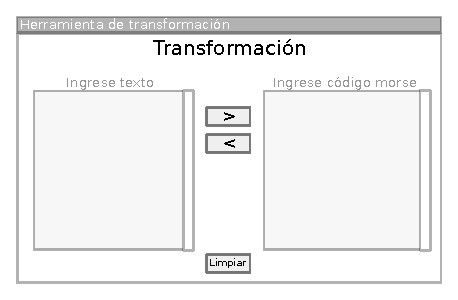
\includegraphics[scale=1]{images/fig-1.pdf}}}
            \caption{Interfaz de usuario}\label{fig:graf-user-mt}
        \end{center}
    \end{figure}

\begin{verbatim}
import java.awt.BorderLayout;
import java.awt.FlowLayout;
import java.awt.event.ActionEvent;
import java.awt.event.ActionListener;
import javax.swing.JButton;
import javax.swing.JFrame;
import javax.swing.JLabel;
import javax.swing.JPanel;
import javax.swing.JScrollPane;
import javax.swing.JTextArea;

public class TranslatorView extends JFrame {

    private JTextArea texto, morse;
    private JButton texto2morse, morse2texto, limpiar;
    private JPanel panelTitulo, panelTexto, panelBotones, panelMorse, panelLimpiar;
    private JScrollPane scrollPaneTexto, scrollPaneMorse;
    
    public TranslatorView() {
        super("Herramienta de transformación");
        initialComponent();
    }

    private void initialComponent() {
        
        texto = new JTextArea(10,15);
        morse = new JTextArea(10,15);
        texto2morse = new JButton(">");
        morse2texto = new JButton("<");
        limpiar = new JButton("Limpiar");
        panelTitulo = new JPanel();
        panelTexto = new JPanel();
        panelBotones = new JPanel();
        panelMorse = new JPanel();
        panelLimpiar = new JPanel();
        scrollPaneTexto = new JScrollPane(texto);
        scrollPaneMorse = new JScrollPane(morse);
        
        setLayout(new BorderLayout());
        
        panelTitulo.setLayout(new FlowLayout(FlowLayout.CENTER, 10, 10));
        panelTitulo.add(new JLabel("Tranformación"));
        add(panelTitulo, BorderLayout.NORTH);

        panelTexto.setLayout(new BorderLayout(10, 10));
        panelTexto.add(new JLabel("Ingrese texto"), BorderLayout.NORTH);
        panelTexto.add(scrollPaneTexto, BorderLayout.CENTER);
        add(panelTexto, BorderLayout.WEST);

        panelBotones.setLayout(new FlowLayout(FlowLayout.LEADING, 10, 40));
        texto2morse.addActionListener(new OyenteTexto2Morse());
        panelBotones.add(texto2morse, BorderLayout.NORTH);
        morse2texto.addActionListener(new OyenteMorse2Texto());
        panelBotones.add(morse2texto, BorderLayout.SOUTH);
        add(panelBotones, BorderLayout.CENTER);
        
        panelMorse.setLayout(new BorderLayout(10, 10));
        panelMorse.add(new JLabel("Ingrese código morse"), BorderLayout.NORTH);
        panelMorse.add(scrollPaneMorse, BorderLayout.CENTER);
        add(panelMorse, BorderLayout.EAST);

        panelLimpiar.setLayout(new FlowLayout(FlowLayout.CENTER, 10, 10));
        limpiar.addActionListener(new OyenteLimpiar());
        panelLimpiar.add(limpiar);
        add(panelLimpiar, BorderLayout.SOUTH);
          
        setSize(400, 400);
        setVisible(true);
        setDefaultCloseOperation(EXIT_ON_CLOSE);
    }
    
    public static void main(String[] args) {
        TranslatorView view = new TranslatorView();
    }
    
    class OyenteTexto2Morse implements ActionListener {

        @Override
        public void actionPerformed(ActionEvent e) {
            morse.setText(TranslatorHelper.text2morse(texto.getText()));
        }
    }
    
    class OyenteMorse2Texto implements ActionListener {

        @Override
        public void actionPerformed(ActionEvent e) {
            texto.setText(TranslatorHelper.morse2text(morse.getText()));
        }
    }
    
    class OyenteLimpiar implements ActionListener {

        @Override
        public void actionPerformed(ActionEvent e) {
            texto.setText("");
            morse.setText("");
        }
    }
}
\end{verbatim}

\end{enumerate}
}
\end{document} 
